\documentclass[11pt]{article}
\usepackage[top=1in,bottom=1in,left=0.5in,right=0.5in]{geometry}
\usepackage{graphicx}
\begin{document}

\title{CS296 Group-06 Project Report : Rube Goldberg Machine Box2D Simulation}
\author{ 
Sagar Jha\\*
110100024\\*
sagarjha@cse.iitb.ac.in\\*\\*
Mridul Garg\\*
110050030\\*
gmridul@cse.iitb.ac.in\\*\\*
Sudipto Biswas \\*
110050048\\*
sudipto@cse.iitb.ac.in\\*\\*
}
\date{\today}
\maketitle

\section{Introduction}
The purpose of the project is to create a Box2D simulation based on the following pre-conceptualised Rube Goldberg machine design\cite{rube_g}.
\begin{center}
\includegraphics[scale=0.4]{design}
\end{center}
The design features many different physical elements like a Newton's cradle like 4-pendulum structure, a gear like structure, two joined pulley system and curved slides. What makes this design interesting is like any other Rube Goldberg machine, the design provides a complicated yet elegant trajectory for the dynamic elements it portrays. The project has tried to follow the original design to its closest approximity. The project differs from the original design in the sense that it ends on a different note. It was learnt that a window cannot be made in Box2D. Thus, an extension of the 2-pulley system was created along with a surprise at the end. \\*
\[Note:\ Run\ the\ simulation\ to\ find\ out\ what\ surprise\ the\ end\ has\ in\ store\]\\* This is a screenshot of the simulation:  
\begin{center}
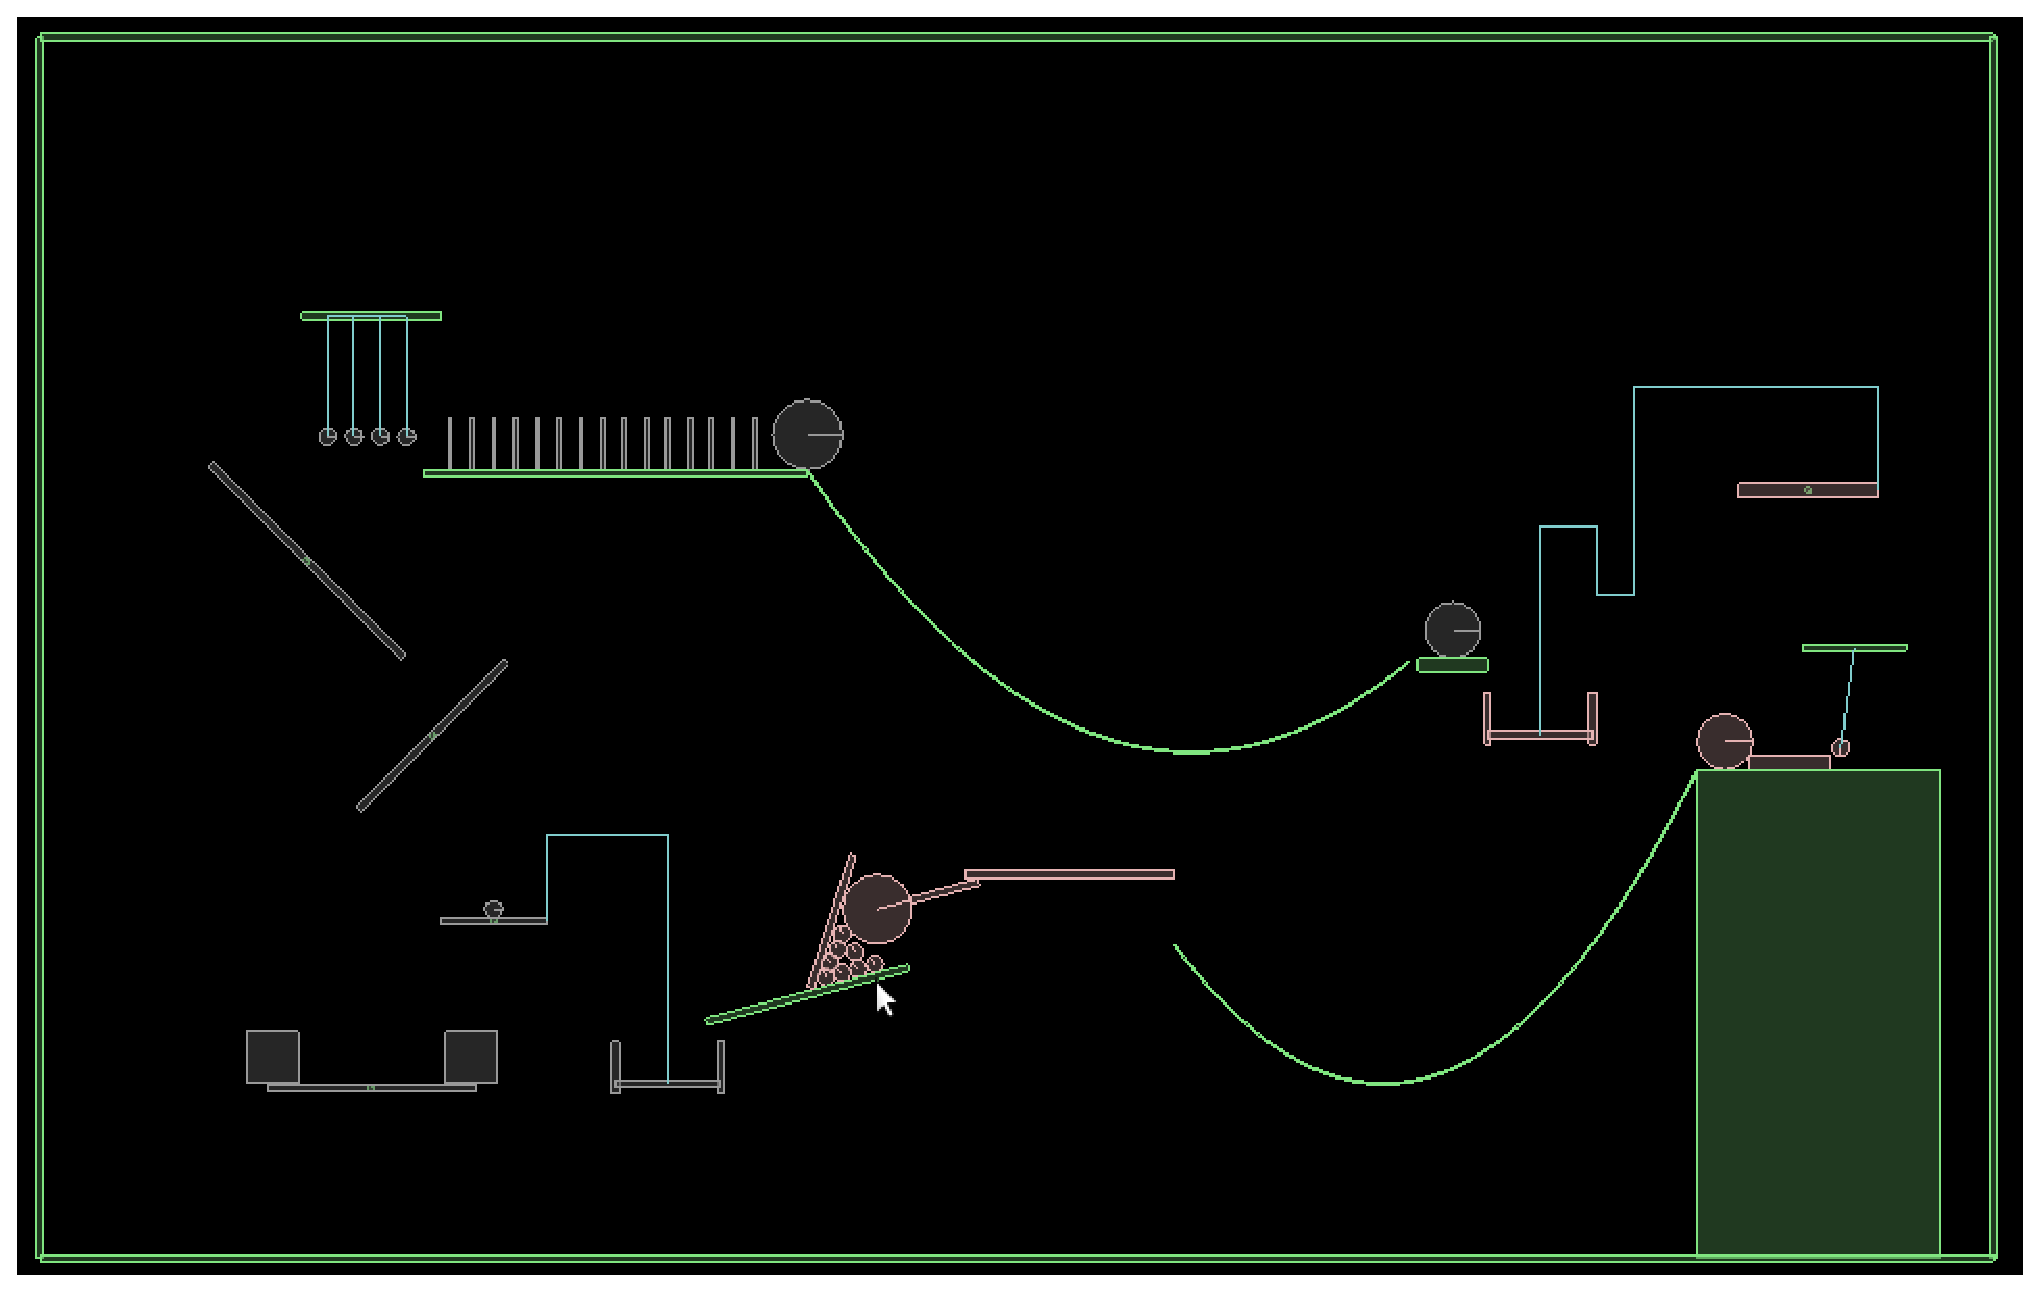
\includegraphics[scale=0.5]{sim}
\end{center}
The next section gives the detailed description of all the physical elements implemented in the project.\\* 
\section{Elements of Simulation}
\subsection{Pendulum}
\begin{center}
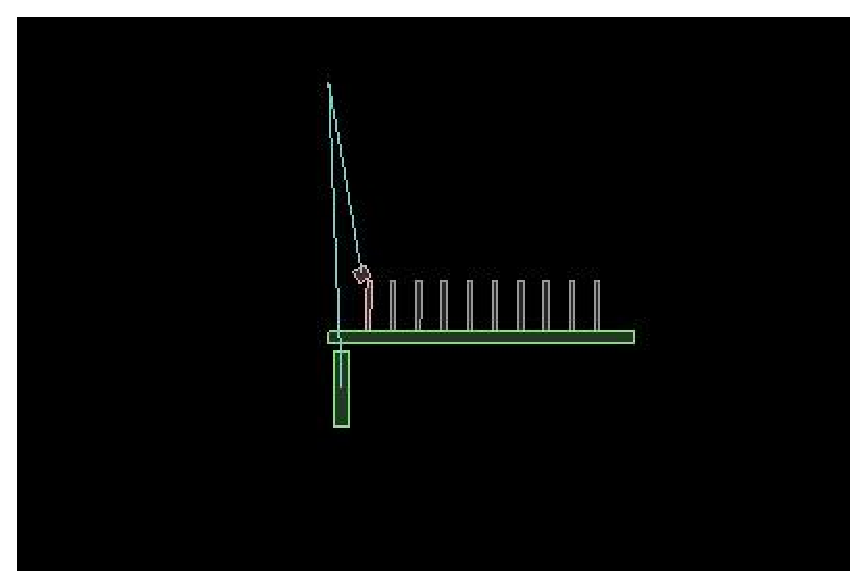
\includegraphics[scale=0.5]{pendulum}
\end{center}
The project simulation consists of 5 pendulums out of which 4 form a Newton's cradle like structure. The bob of the one independent pendulum initiates the Rube Goldberg machine.
\subsection{Pulley System}
The project simulation consists of two pulley system out of which one pulley system is three pulleys joined together i.e. a triple pulley system.
\begin{center}
\includegraphics[scale=0.5]{pulley1}
\includegraphics[scale=0.5]{pulley2}
\end{center}
\subsection{Hinged Rod System}
The project simulation consists of four such hinged rod systems out of which two of them are connected to pulley systems. The hinged rods provide free rotation of the rods about the hinges and when connected to the pulleys can trigger required simulation.
\begin{center}
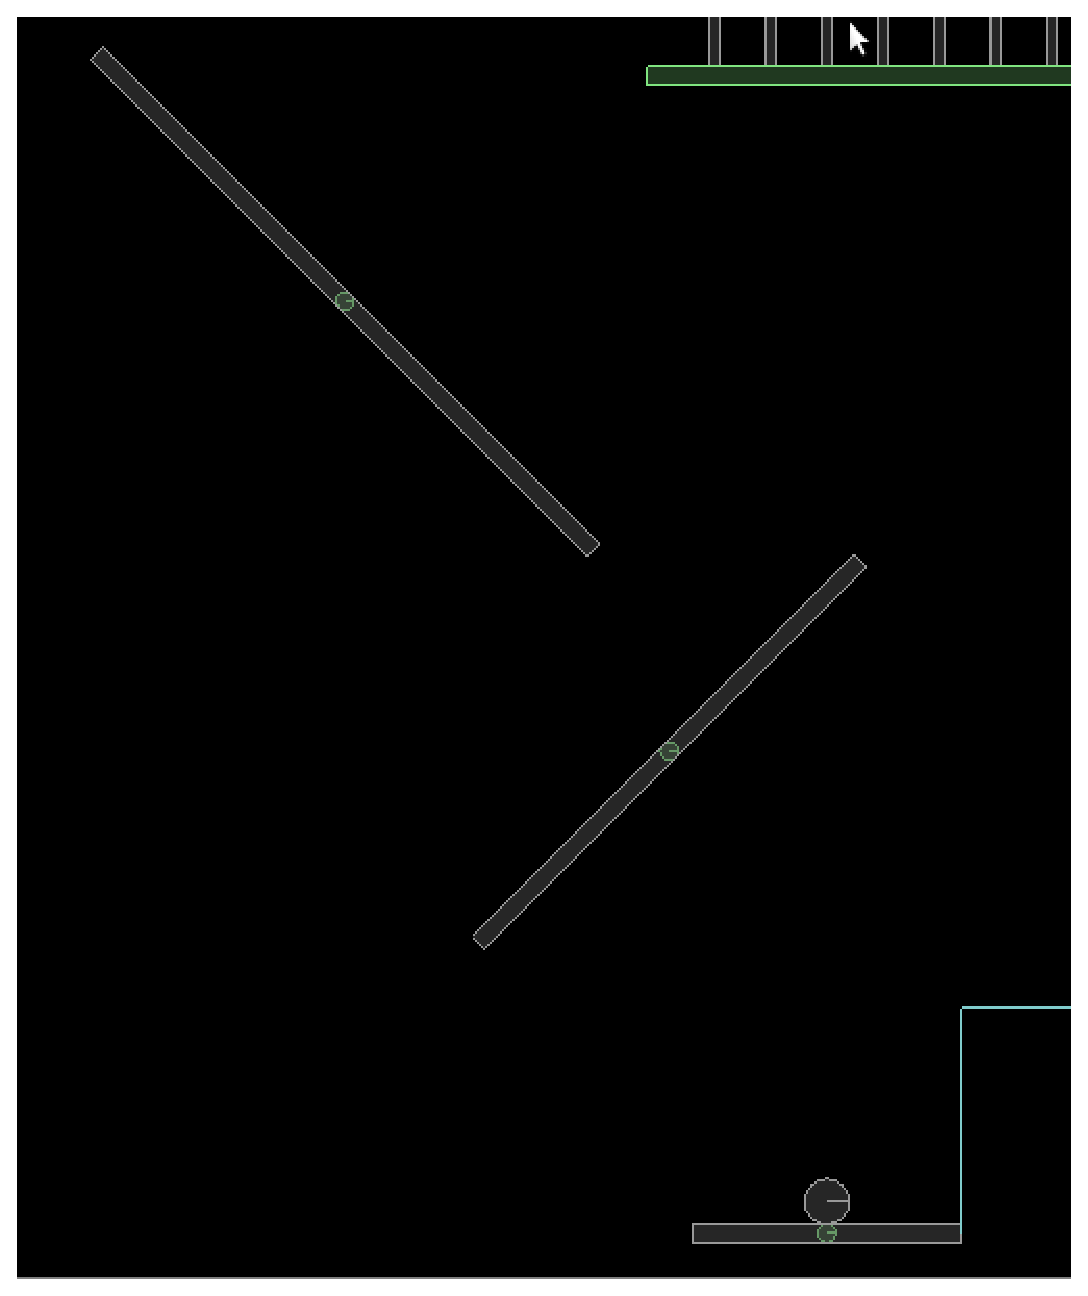
\includegraphics[scale=0.5]{hinge}
\end{center}
\subsection{Gear System}
The project simulation consists of a gear like system in which there is a rotating disc hinged at center and two rods attached to it. One rod is attached in such a way that it holds a collection of small balls in an inclined ground. As soon as the other rod is disturbed or hit by a dynamic object, the other rod holding the balls get disturbed and let the collection of balls it was holding to fall which carries on with the trajectory.
\begin{center}
\includegraphics[scale=0.5]{gear}
\end{center} 
\subsection{Domino System}
The project simulation consists of a long dominoes system containing an array of equally spaced 15 dominoes which are initially stable and standing on a particular ground in the simulation. The 4-pendulum system disturbs the left most domino which in turn takes down all the dominoes one by one and gives velocity to a sphere at the other end.
\begin{center}
\includegraphics[scale=0.5]{domino}
\end{center}
\subsection{Inclined Curved Plains}
The project simulation contains two parabolic inclined curved paths. The inclined paths provide an interesting trajecting for the spheres in the simulation to proceed. The curved paths have been created by building tiny tiny ground (fixed) strips together in a loop along the equation of a parabola. With the appropriate limits and the width and angle of inclination of each such tiny ground strip, its been possible to create the curved planes so realistically. 
\begin{center}
\includegraphics[scale=0.3]{curve1}
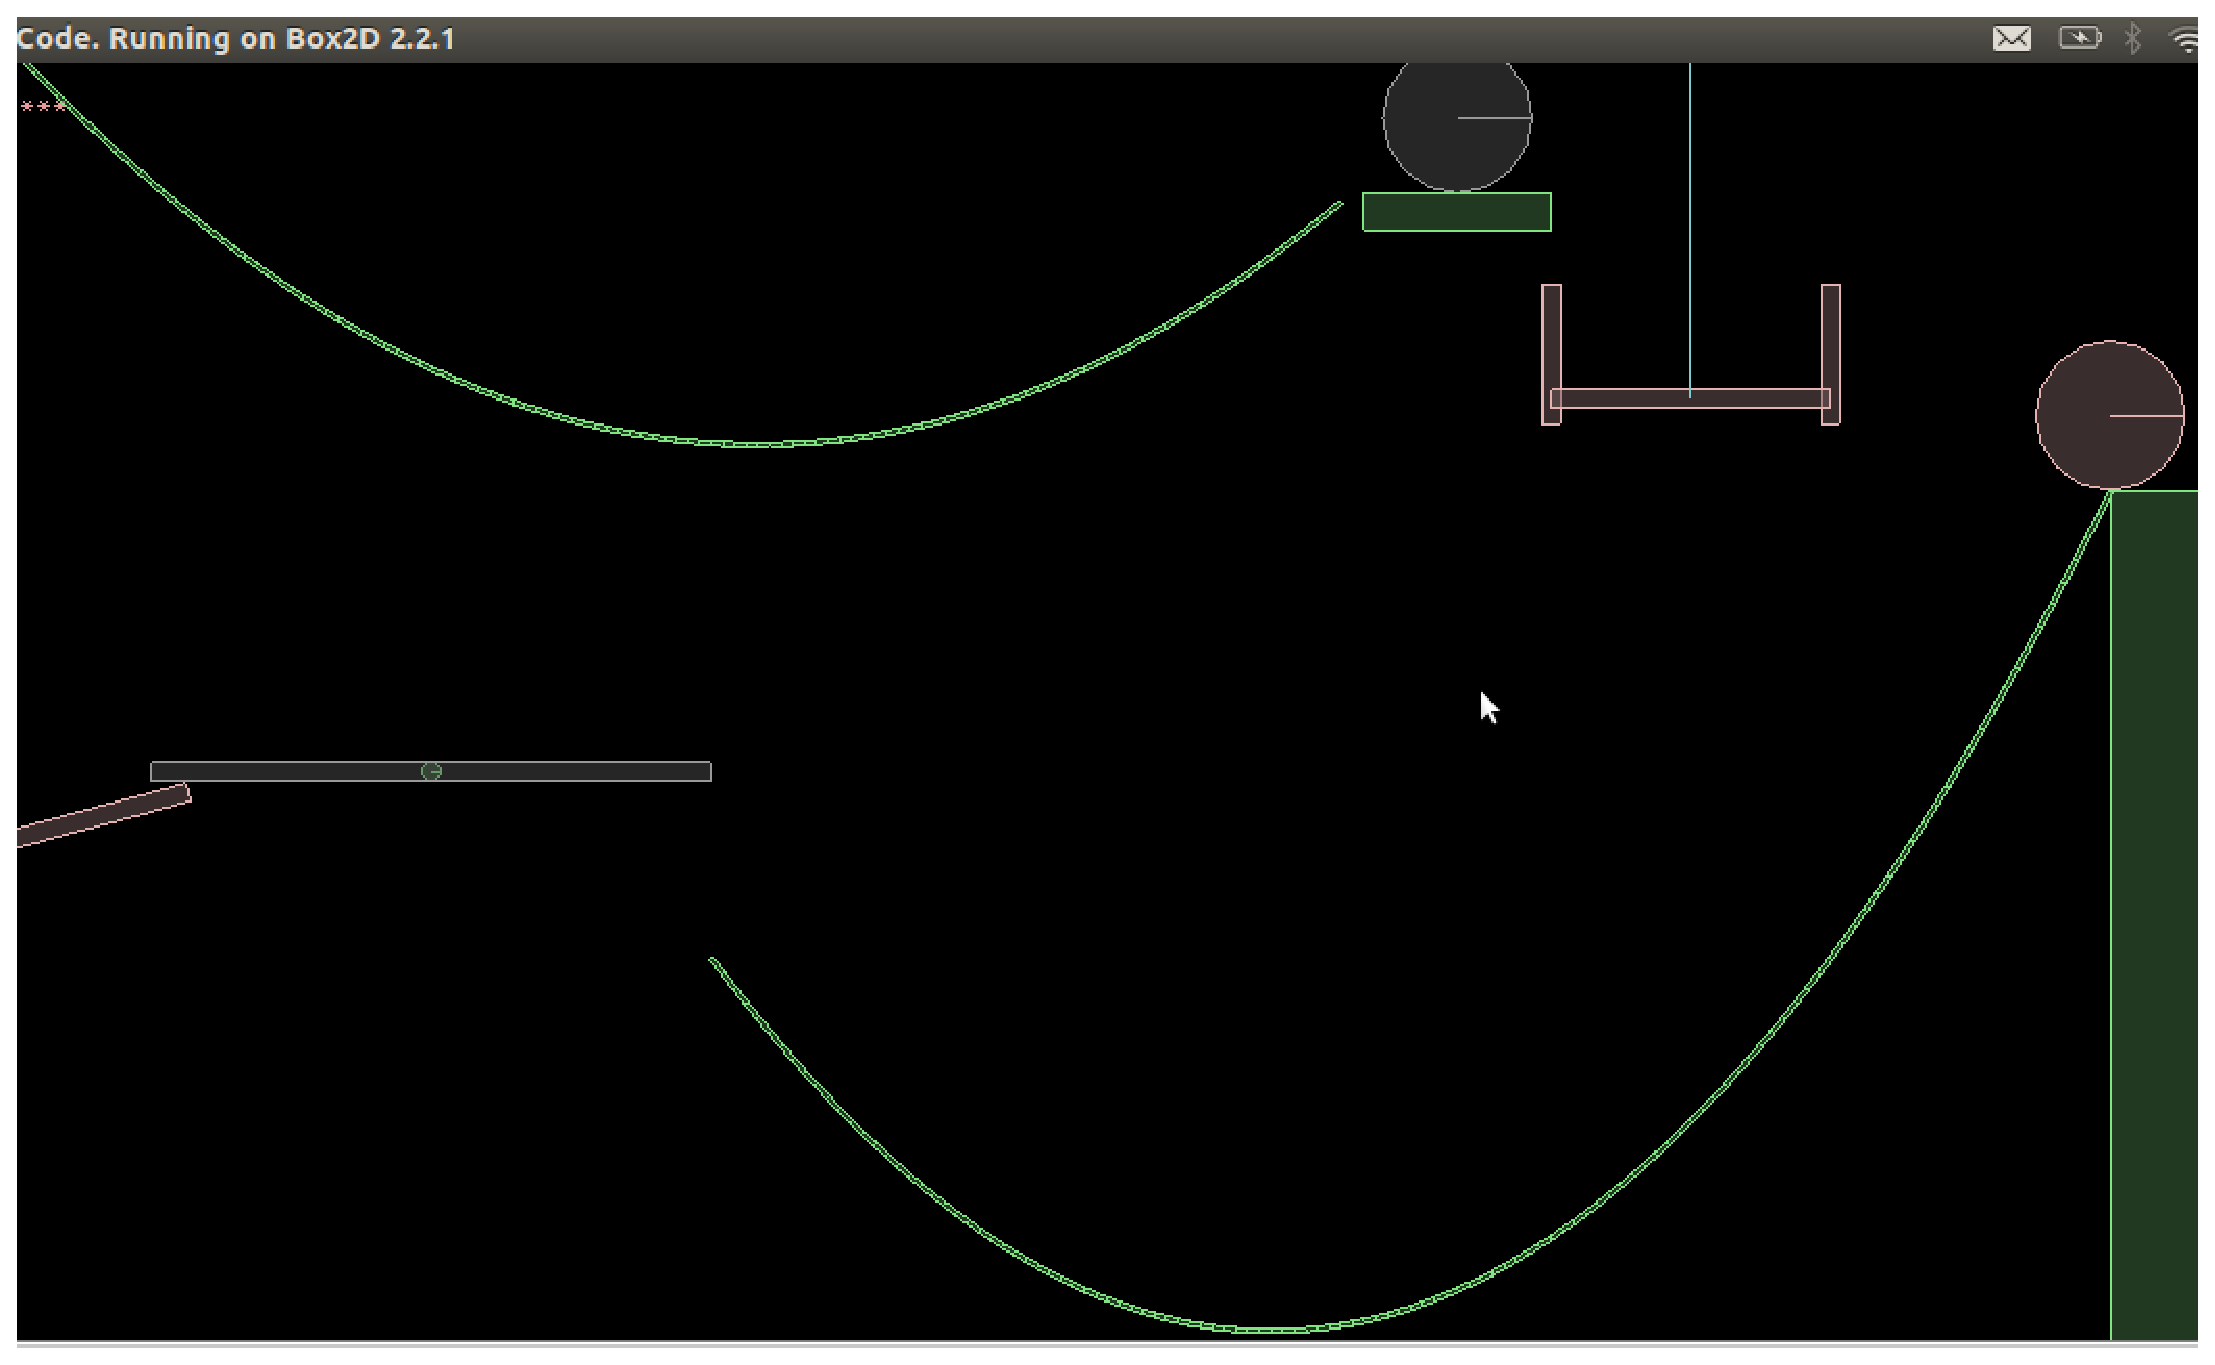
\includegraphics[scale=0.3]{curve2}
\includegraphics[scale=0.3]{curve3}
\end{center}
\subsection{Other Dynamic Bodies : Blocks and Spheres}
Other than all the other systems/elements explained till now, there is left all the dynamic bodies which actually translates and rotates all through the simulation to drive the Rube Golberg machine throughout. These dynamic bodies are free to both translate and rotate, ie they have 5 degrees of freedom. Such dynamic bodies that are present in the project simulation are cubical boxes and spheres. Many spheres are there present throughout the simulation canvas. There are two spheres which move on the curved paths and many small spheres to drive the pulley systems. The cubical boxes or blocks are there to hit and drive the hinged rods.
\begin{center}
\includegraphics[scale=0.5]{sphere}
\end{center}  
\section{Simulation Analysis}
\subsection{Plot 01 : Step time and Total Loop time averaged over Reruns}
\begin{center}
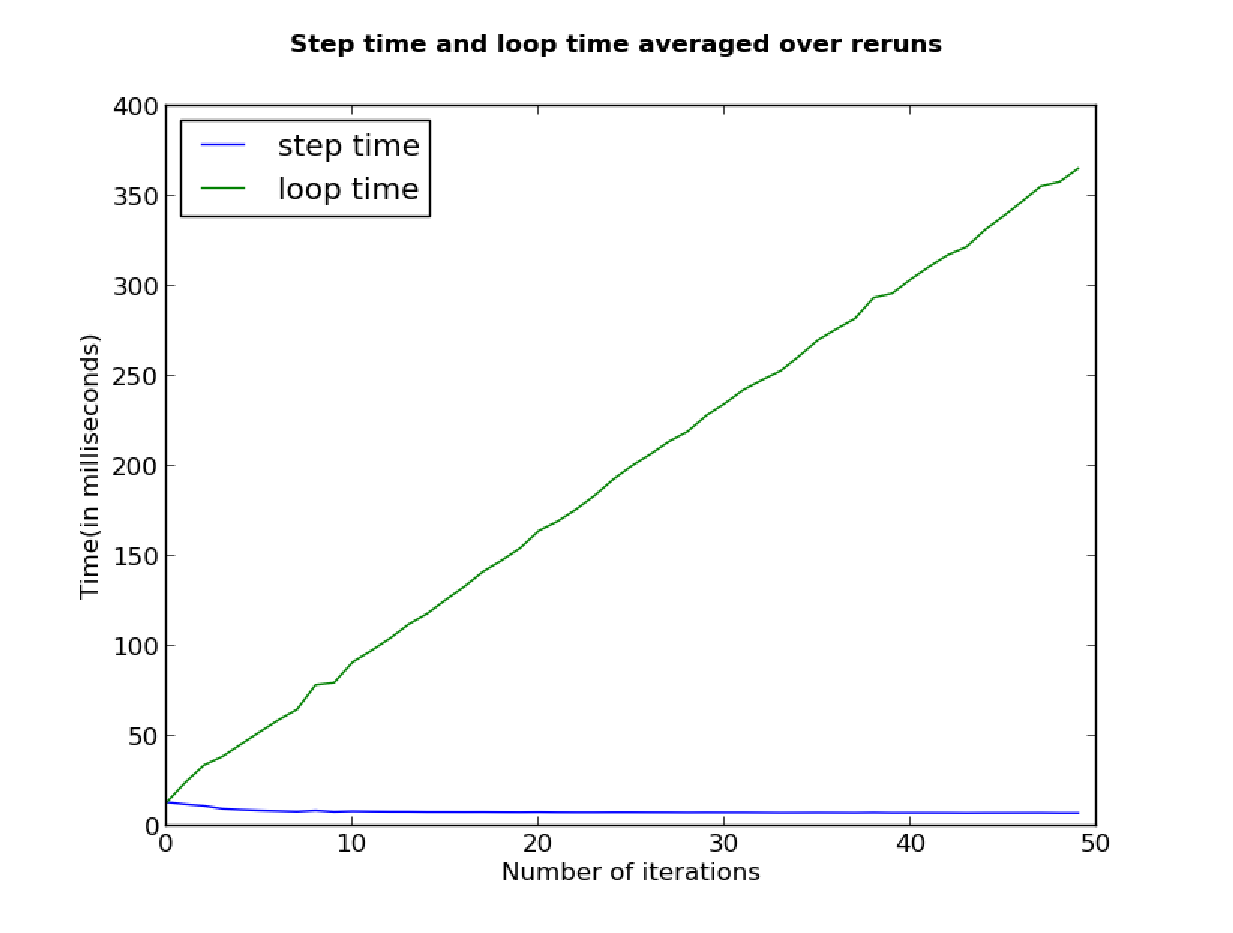
\includegraphics[scale=0.5]{plot01}
\end{center}
1.\ Loop time is greater than the Step time at all points except the first point where both are equal.
\\* 2.\ Total Loop time increases with the number of iterations whereas the Step time stays nearly constant or slightly decreases. \ \ This is because the loop executes iteration times but the step time is averaged over total iterations.
\subsection{Plot 02 : Step time, Velocity update time, Position update time and Collision time averaged over Reruns}
\begin{center}
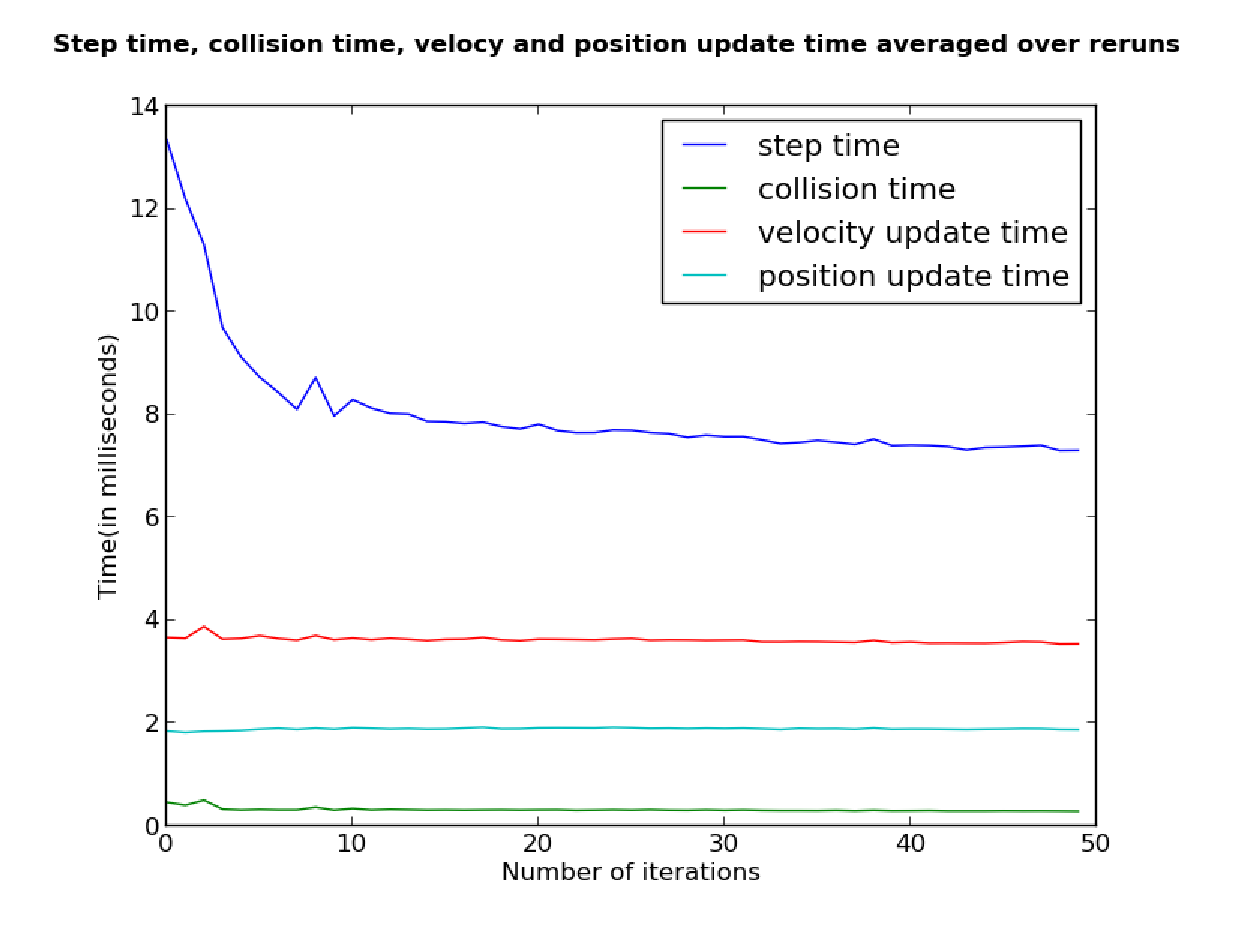
\includegraphics[scale=0.5]{plot02}
\end{center}
1.\ Step time \textgreater \ velocity update time \textgreater \ position update time \textgreater \ collision time
\\*2.\ Each of these decrease slightly with the number of iterations
\\*3.\ The time taken to update velocity is highest becuase it involves more calculations than the other two.
\subsection{Plot 03 : Step time and Loop time averaged over Iterations}
\begin{center}
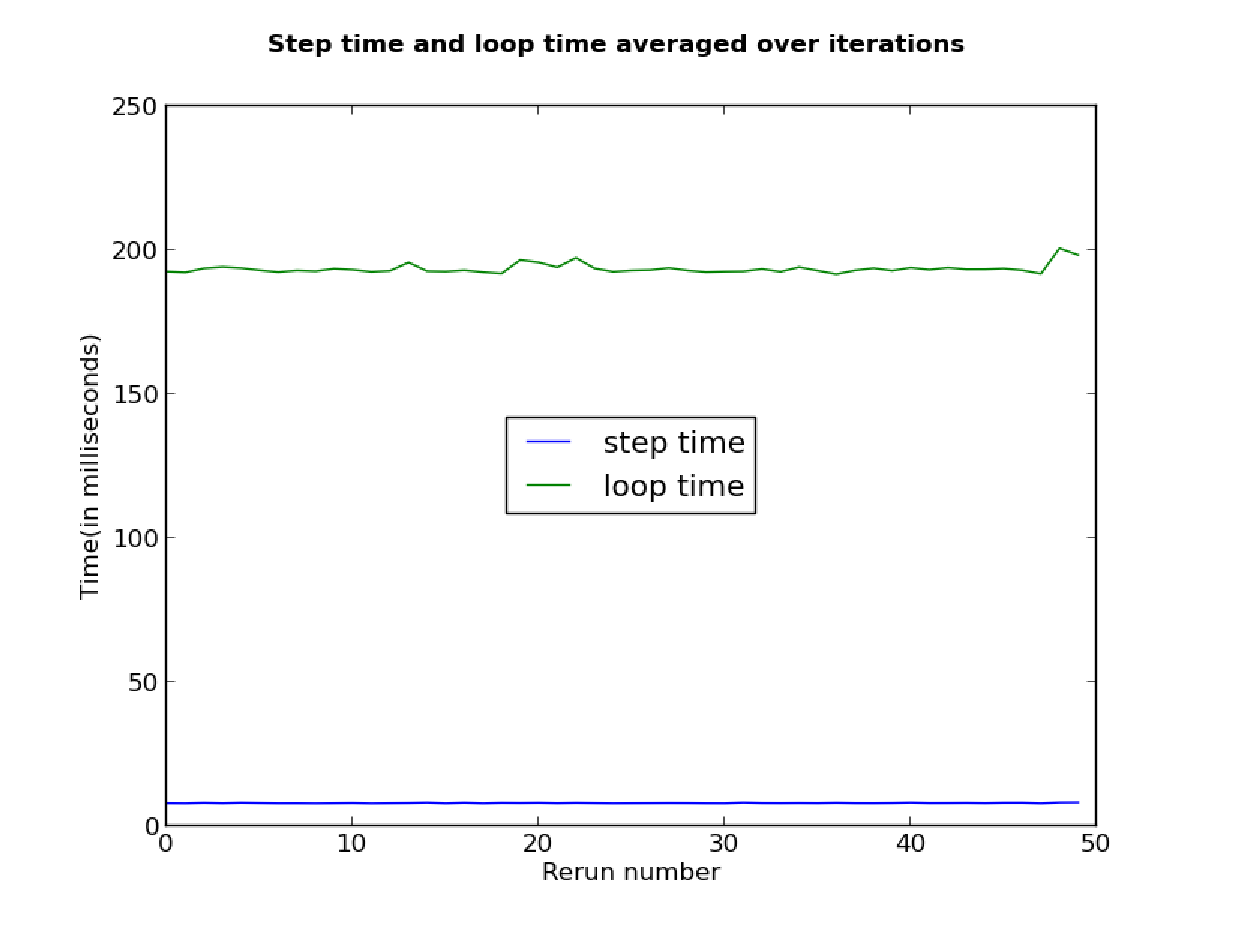
\includegraphics[scale=0.5]{plot03}
\end{center}
Since, there is no difference among the reruns, Step time and Loop time are very closely deviated about the average with the rerun number.
\subsection{Plot 04 : Step time, Velocity update time, Position update time and Collision time averaged over Iterations}
\begin{center}
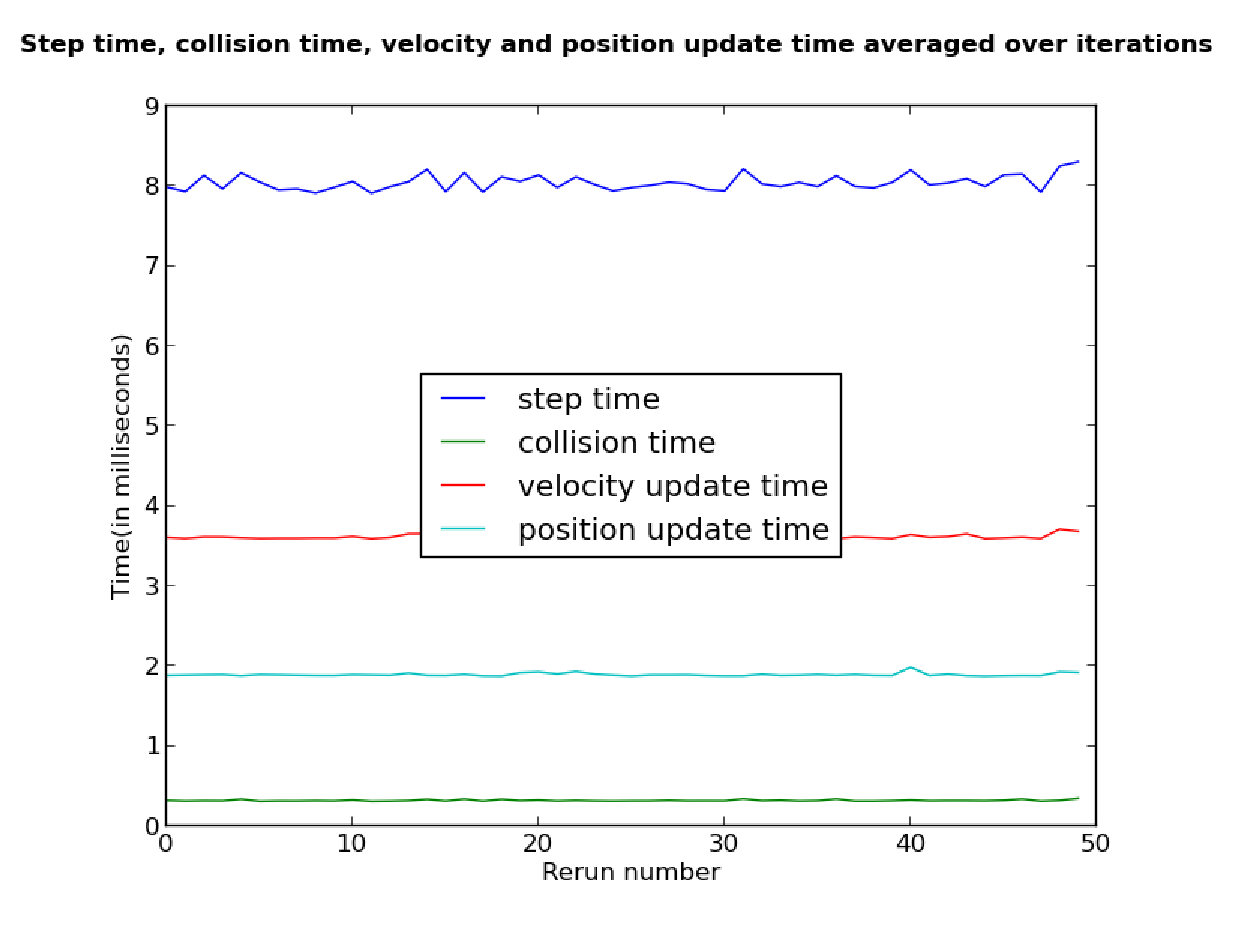
\includegraphics[scale=0.5]{plot04}
\end{center}
Same is the case with this plot of collision time, velocity update time and position update time. Like the previous plot, all of them are slightly deviated about their respective averages with the rerun number.
\subsection{Plot 05 : Deviation in all the Time measurements}
\begin{center}
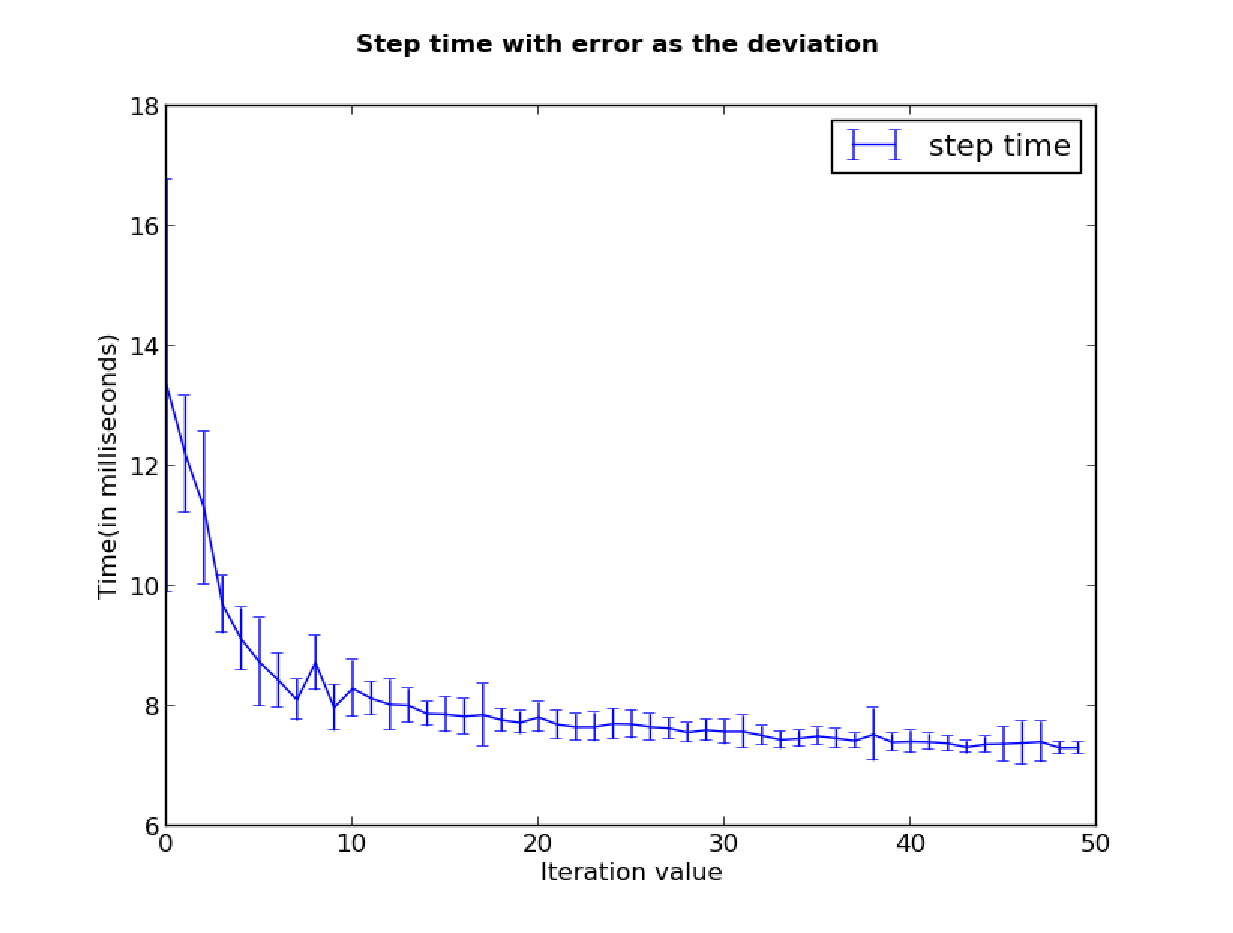
\includegraphics[scale=0.5]{plot05}
\end{center}
1.\ Deviation of Step time \textgreater \ Velocity update time \textgreater \ Position update time \textgreater \ Collision time
\\*2.\ This together with the second plot shows that the percentage deviation of all the three is nearly equal.
\subsection{Plot 06 : Frequency Distribution and Cumulative Distribution}
\begin{center}
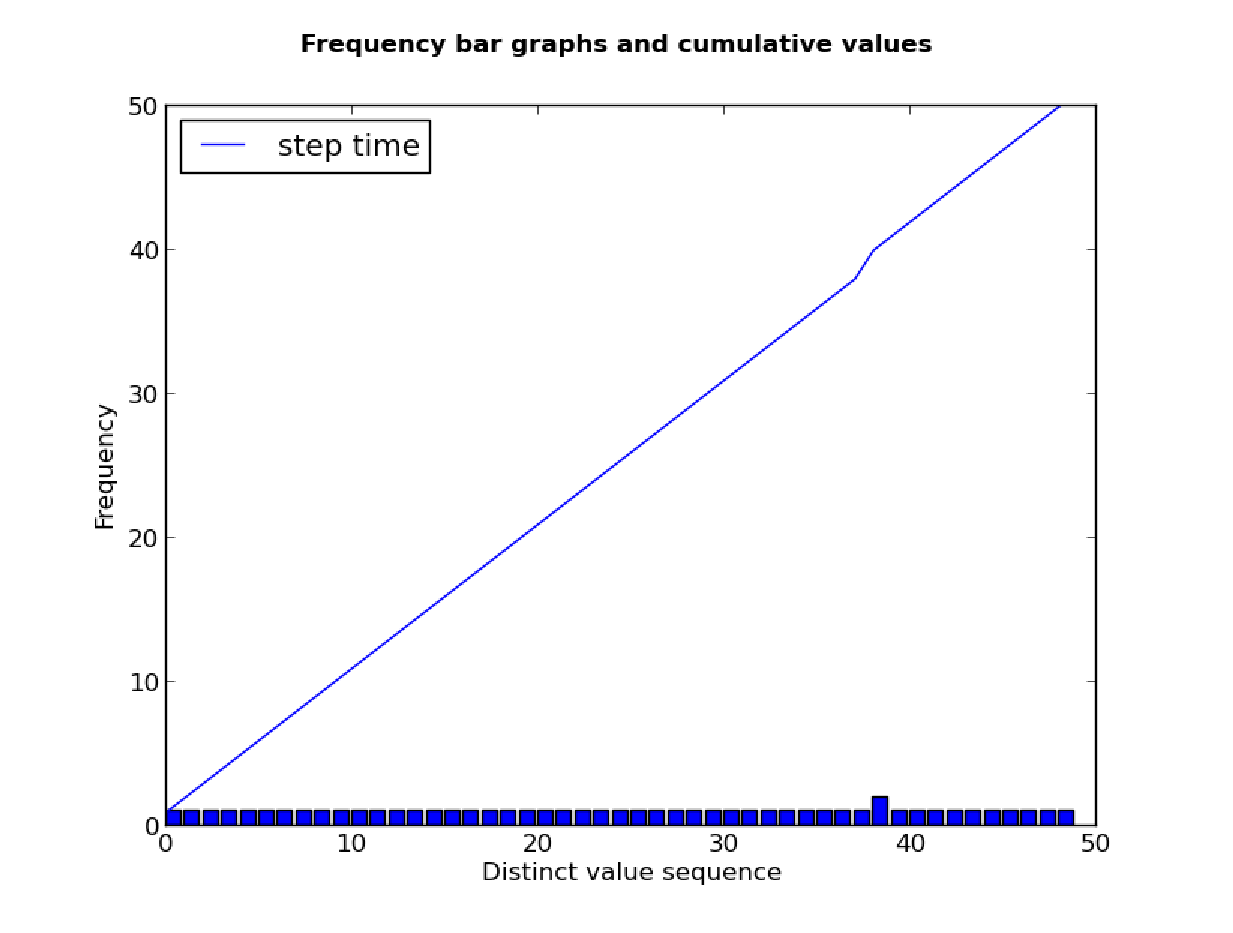
\includegraphics[scale=0.5]{plot06}
\end{center}
\section{Simulation Performance}
In debug mode, the functions SolveVelocityConstraints, operator -, and b2Cross take up the majority of the time whereas in release mode, the functions SolveVelocityConstraints and SolvePositionConstraints take up most of the time. Also, in release mode, the time taken is nearly 1/5th of the time taken in debug mode (175 ms per simulation compaired to 875 ms)
\begin{center}
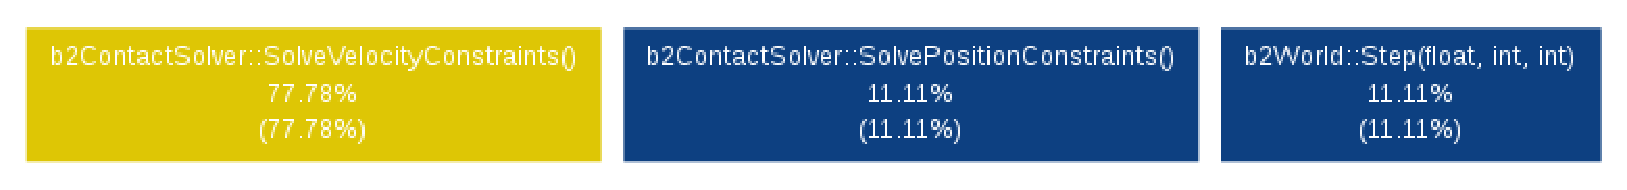
\includegraphics[scale=0.5]{release}
\end{center}
\begin{center}
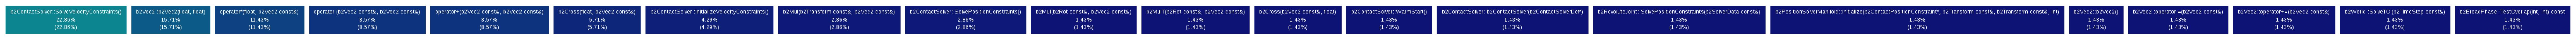
\includegraphics[scale=0.05]{debug}
\end{center}
\section{Conclusions}
The project thus succeeds in presenting a clean simulation which 
\bibliographystyle{plain}
\bibliography{mybib}
\end{document}
